\section{Related Work}

%\subsection{Function Merging through Sequence Alignment} \label{related:salssa}

%SalSSA~\cite{rocha20} has a search strategy for pairing similar functions for merging but avoiding a prohibitively expensive quadratic number of merging attempts.
%The purpose of the search strategy is to avoid a quadratic exploration that attempts to merge all possible pairs of functions.
%All three techniques use a ranking strategy based on the \textit{fingerprint} of the functions to evaluate their similarity.
%They start by precomputing and caching fingerprints for all functions.
%The fingerprint is a fixed-size vector that summarizes the content of the function.
%To this end, the fingerprint consists of a map of instruction opcodes to their frequency in the function.
%While functions can have several thousands of instructions, an IR usually has just a few tens of opcodes, e.g., the LLVM IR has only about 68 different opcodes.

%The fingerprint representation allows us to compare functions using a simple distance metric, such as the Manhattan distance.
%For a given reference function, all other functions are ranked based on the distance of their fingerprints.
%The candidate function with the smallest distance will be used for a merging attempt.

%By comparing the opcode frequencies of two functions, we are able to estimate
%the best case merge, which would happen if all instructions with the same opcode could match.
%This is a very optimistic estimation. It would be possible only if instruction types and order
%did not matter. We refine it further by estimating another best case merge, this time based
%on type frequencies, which would happen if all instructions with the same data type could match.

%Since the fingerprint of functions have fixed size, i.e., the number of instruction opcodes, the distance between two functions can be computed in constant time.

% \begin{figure}[h]
%   \centering
%   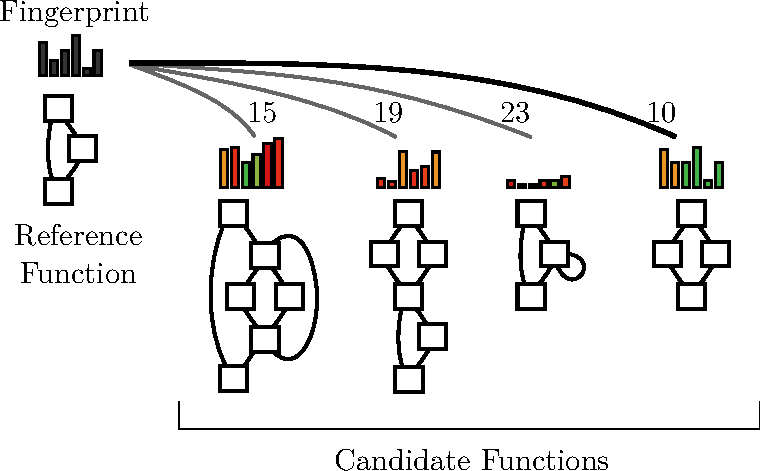
\includegraphics[width=\linewidth]{figs/hyfm-ranking.pdf}
%   \caption{.}
%   \label{fig:hyfm-ranking}
% \end{figure}


%\subsection{Merging Similar Functions}

Compiler-based code size reduction is important for fitting large programs to resource-limited embedding devices. Previous approaches reduce code size by replacing a code segment with a smaller, semantically- equivalent implementation~\cite{massalin87,tanenbaum82}, or removing or combining redundant
code~\cite{cocke70,knoop94,ernst97,cooper99,debray00,chen03,loki04}. Function merging falls into the latter category. 


The function merging technique presented in \cite{edler14} restricts merging to nearly identical functions. They only allow for pairs of corresponding instructions to differ if they still have equivalent data type.


A phi-node is used to unify the mismatching instructions as a single named value.
Every use of the mismatching instructions will refer to their phi-node.
Two instructions match if they have the same opcode with equivalent data types and operands.
Note that no operand selection is performed.
Even if two instructions differ only on their operands, they are classified as mismatching, and a branch is created.

% \begin{figure}[h]
%   \centering
%   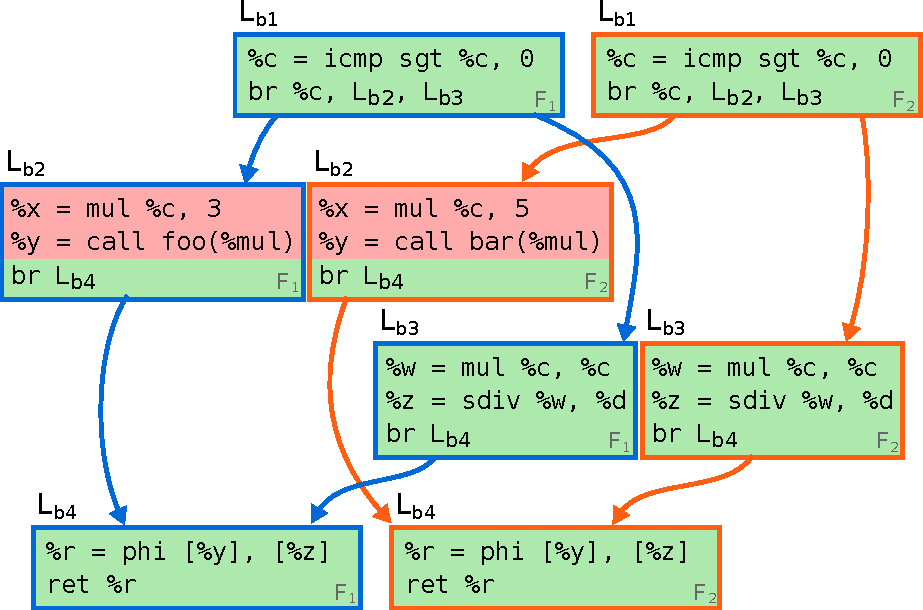
\includegraphics[width=\linewidth]{figs/soa-example-1.pdf}
%   \caption{.}
%   \label{fig:soa-example-1}
% \end{figure}

Except for mismatching pairs of instructions, the two functions must have identical function types, i.e., they must have the same return type and list of arguments, identical CFGs, with corresponding basic blocks having the same number of instructions.

** however, these instructions must define names representing the same data type.

% \begin{figure}[h]
%   \centering
%   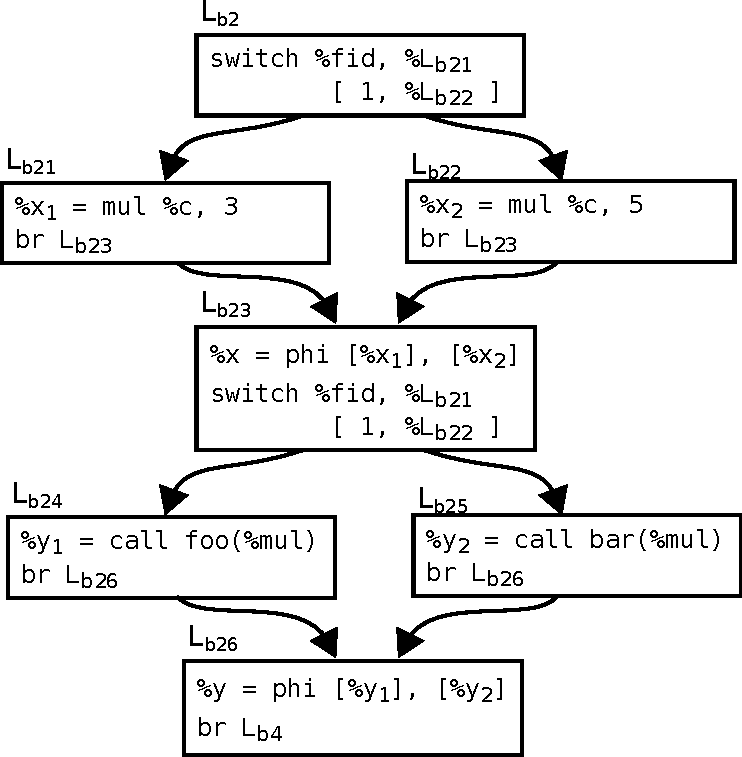
\includegraphics[width=0.8\linewidth]{figs/soa-example-2.pdf}
%   \caption{.}
%   \label{fig:soa-example-2}
% \end{figure}


